\documentclass[a4paper,11pt,oneside]{book}
\usepackage[margin=1.2in]{geometry} 

%% Math/Definition/Theorem/Algorithm packages settings 
\usepackage[cmex10]{amsmath}
\usepackage{amssymb}
\usepackage{amsthm}
\newtheorem{mydef}{Definition}
\newtheorem{mytherm}{Theorem}

%% Algorithms/Code Listing environment settings  - 
\usepackage{float}
\usepackage{pygmentex}
\usepackage{algorithm}
\usepackage{algpseudocode}
\renewcommand{\algorithmicrequire}{\textbf{Input:}}
\renewcommand{\algorithmicensure}{\textbf{Output:}}
\usepackage[utf8]{inputenc}
\usepackage{listings}
\usepackage{xcolor}
\definecolor{codegreen}{rgb}{0,0.6,0.1}
\definecolor{codegray}{rgb}{0.5,0.5,0.5}
\definecolor{codeblue}{rgb}{0.10,0.00,1.00}
\definecolor{codepurple}{rgb}{0.58,0,0.82}
\definecolor{backcolour}{rgb}{1.0,1.0,1.0}
\lstdefinestyle{mystyle}{
    backgroundcolor=\color{backcolour},   
    commentstyle=\color{codegreen},
    keywordstyle=\color{codeblue},
    numberstyle=\tiny\color{codegray},
    stringstyle=\color{codepurple},
    basicstyle=\ttfamily\footnotesize,
    breakatwhitespace=false,         
    breaklines=true,                 
    captionpos=b,                        
    keepspaces=true,                 
    numbers=left,                    
    numbersep=5pt,                  
    showspaces=false,                
    showstringspaces=false,
    showtabs=false,                  
    tabsize=2,
    frame=none
}
\lstset{style=mystyle}

%% Graphics/Figures environment settings
\usepackage{graphicx}
\usepackage{subfigure}
\usepackage{caption}
\usepackage{lipsum}

%% Table environment settings
\usepackage{multirow}
\usepackage{rotating}
\usepackage{makecell}
\usepackage{booktabs}

%% List of Abbreviations settings
% TODO: remove this (causes hbox warnings)
\hbadness=99999
\hfuzz=9999pt
\usepackage{enumitem}
\newlist{abbrv}{itemize}{1}
\setlist[abbrv,1]{label=,labelwidth=1in,align=parleft,itemsep=0.1\baselineskip,leftmargin=!}

%% Bibliography/References settings   - Harvard Style was used in this report
\usepackage[backend=bibtex]{biblatex} %Imports biblatex package
\addbibresource{references.bib}
\usepackage[hidelinks]{hyperref}
\renewcommand{\bibname}{References} % DO NOT remove or switch of 

%% Appendix settings     
\usepackage[toc]{appendix}

%% Document
\begin{document} 
    \frontmatter
    
    \begin{titlepage}      
        \begin{center}
            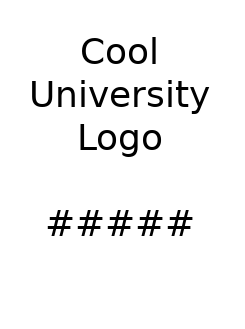
\includegraphics[width=0.3\textwidth]{figures/uni-logo.png}\\[0.5cm]
            {\LARGE *** University\\[0.5cm]
            Department of ******}\\[2cm]
            \linespread{1.2}\huge {
                Your title
            }
            \linespread{1}~\\[2cm]
            {\Large 
                Your Name
            }\\[1cm] 

            {\large 
                \emph{Supervisor:} Supervisor's name}\\[1cm]
            
            \large subtitle \\[0.3cm] 
            \vfill
            
            \date{September 2022}
        \end{center}
    \end{titlepage}

    % Declaration
    \newpage
    \thispagestyle{empty}
    \chapter*{\Large Declaration}
        I, ****, here by .... \\
    \noindent
    This report may be shared with ...
    ~\\[1cm]
    \begin{flushright}
        Your Name
    \date{September 2022}
    \end{flushright}

    % Abstract and Acknowledgement
    \chapter*{\center \Large  Abstract}
Abstract Abstract Abstract Abstract Abstract Abstract Abstract Abstract Abstract Abstract Abstract Abstract Abstract Abstract Abstract Abstract Abstract Abstract Abstract Abstract Abstract Abstract Abstract Abstract Abstract Abstract Abstract Abstract Abstract Abstract Abstract Abstract Abstract Abstract Abstract Abstract Abstract Abstract Abstract Abstract Abstract Abstract Abstract Abstract Abstract Abstract Abstract Abstract Abstract Abstract Abstract Abstract Abstract Abstract Abstract Abstract Abstract Abstract Abstract Abstract Abstract Abstract Abstract Abstract Abstract Abstract Abstract Abstract Abstract Abstract Abstract Abstract Abstract Abstract Abstract Abstract Abstract Abstract Abstract Abstract Abstract.

~\\[1cm]
\noindent
\textbf{Keywords:} key1, key2, key3

   
    % Acknowledgement
    \chapter*{\center \Large  Acknowledgements}
I would like to express my gratitude to ...
   
    
    % Contents, list of figures, list of tables
    \tableofcontents
    \listoffigures
    % \listoftables
    % \chapter*{List of Abbreviations}
\chaptermark{List of Abbreviations}
\begin{abbrv}
    \item[GNU] GNU's Not Unix
\end{abbrv}

    
    % Main chapters and sections
    \mainmatter
    
    \chapter{Introduction}
\label{ch:into}
Introduction

    \chapter{Conclusion}
\label{ch:con}
Conclusion

    \printbibliography[heading=bibintoc,title={References}]
\end{document}
